\section{Performance Experiments}

We will conduct several performance experiments based on our proposed models. The quantitative analysis we may do are as follows:
\begin{itemize}
    \item To make our simulation results more representative, we will introduce several airline routes on behalf of different city scales. By collecting the number of people infected with COVID-19 and the number of susceptible and recovered people in different cities at the same time periods, we will use SI, SIR, SIRS, and SEIR models to characterize the spread of epidemics in different cities in the form of differential equations. By comparing with actual data, we will select the best-fitting infection simulation model.
    \item After obtaining the infection rate, we will determine the appropriate number of flights through the established optimization model, so as to maximize the city's utility while reducing the risk of infection as much as possible. The optimization results of different cities may vary, because the weight of routes and infection rates are different. In the most severe case of epidemic, the optimization result is likely to be a route suspension.
    \item Under the above model, we will make a decision of whether the target city will cut flights based on the current epidemic situation. By comparing with the "Five One" policy implemented by CAAC, we will analyze whether our proposed network optimization model is reasonable, and further put forward how to better formulate relevant policies through the model.
\end{itemize}

\subsection{General Settings}
We have chosen nine cities with the highest annual flight movements in 2019 and Wuhan, the pandemic center, to construct our airline network with pairwise combinations, as shown in Table 1. In particular, we only consider Beijing Capital International Airport and Shanghai Pudong International Airport since these two airports occupy more market shares in the corresponding city. 
\begin{table}[H]
    \centering
    \caption{The city group for proposed model}
    % \footnotesize
    \setlength{\tabcolsep}{1pt}
    \begin{tabular}{ccccc}
        \toprule
         1 & 2 & 3 & 4 & 5 \\
         Beijing & Shanghai & Guangzhou & Chengdu & Shenzhen \\
        \toprule
        6 & 7 & 8 & 9 & 10 \\
        Kunming & Xi'an & Chongqing & Hangzhou & Wuhan \\
        \bottomrule
    \end{tabular}
    \label{table1}
\end{table}
As mentioned in section 3.1, we need data from annual passenger flow and annual GDP to represent the weighted value of selected two city-pairs and the average number of infections and cured patients to show the rate of infections. Here we list related data for any given date in table 2. Several other statistic datasets, i.e. the maximum capacity, weighted value, severity of the epidemic and the rate of infection of the corresponding $10\times 10$ city-pairs are calculated in table 3 and table 4, shown in the appendix.

\begin{spacing}{2}
\begin{table}[H]
    \centering
    \caption{Datasets of $\{g_i, t_i, I_i, E_i\}$ (Apr. $16^{\rm th}$)}
    \setlength{\tabcolsep}{5pt}
    % \footnotesize
    \begin{tabular}{c|c|c|c|c}
        \toprule
         City $i$ & $g_i$ / trillion & $t_i$ / million & $I_i$ & $E_i$ \\
         \toprule
         1 & 3.54 & 100.2 & 593  & 50 \\
         2 & 3.82 & 76.0 & 628 & 496 \\
         3 & 2.36 & 72.7 & 499 & 449 \\
         4 & 1.70 & 55.3 & 165 & 155 \\
         5 & 2.69 & 52.3 & 459 & 429 \\
         6 & 0.65 & 48.0 & 53 & 53 \\
         7 & 0.93 & 46.9 & 120 & 117 \\
         8 & 2.36 & 44.6 & 579 & 576 \\
         9 & 1.54 & 39.8 & 181 & 181 \\
         10 & 1.62 & 26.8 & 50008 & 47283 \\
        \bottomrule
    \end{tabular}
    \label{table2}
\end{table}
\end{spacing}
In order to make our experimental results more reasonable, we have collected
the target cities' airline capacities in the past six months from Flightera\footnote{\url{https://www.flightera.net/en/}}, a website dedicating to provide accurate flight dynamic information for customers, and choose the maximum value as $c_{ij}^{max}$. As illustrated in Figure 2, we can see that there is a certain symmetry in the maximum number of flights between any two city pairs. In general, cities with more significant values have more access to other cities, as row 1 and column 1 represent the capital city Beijing. Besides, there are no flights on the diagonal since we require departure airport and destination airport are different in our model.


\begin{figure}[H]
    \centering
    \includegraphics[width=0.85\columnwidth]{pic/c_ij_max.eps}
    \caption{$c_{ij}^{max}$ from targeted city $i$ and city $j$}
    \label{fig:my_label}
\end{figure}


\subsection{Performance}
In this section, we focus on analyzing on our experimental results based on our network optimization model. In particular, we emphasize on three aspects, such as epidemic severity, the maximum airline capacity and the relaxation parameters, and analyze whether our optimized results will change when considering different modeling factors. 
\subsubsection{Relationship between $c_{ij}^* / c_{ij}^{max}$ and $S_i$}
% \begin{itemize}
%     \item Relationship between decsion making $c_{ij}^* / c_{ij}^{max}$ and the severity of epidemic $S_i$
% \end{itemize}
From section 4.1, we have given related required datasets of our model in Apr.$16^{\rm th}$. As represented in Figure 3, we regard $c_{ij}^* / c_{ij}^{max}$ as our decision variable variation. It's obvious that the more severe the pandemic in any given city becomes, the smallest airline capacity it will have. Note that there exists no flight route between Shanghai and Hangzhou, airline capacity remains zero. Without loss of generality, we consider another date which represents different levels of severity, shown in figure 3 (a). We can easily find out there are 
obvious difference in some cities less affected by the epidemic.

\begin{figure}[H]
    \centering
    \subfigure[Mar. 27$^{\rm th}$]{
        \includegraphics[width=0.46\columnwidth]{pic/decision_3-27_T_1000_ep_0dot6.eps}
    }
    \subfigure[Apr. 16$^{\rm th}$]{
        \includegraphics[width=0.46\columnwidth]{pic/decision_4-16_T_1000_ep_0dot6.eps}
    }
    \caption{Decision making $c_{ij}^* / c_{ij}^{max}$ of different date with different epidemic severity $\{S_i\}$ ($\epsilon=0.6,T=1000$)}
    \label{fig:my_label}
\end{figure}



\subsubsection{Relationship between $c_{ij}^* / c_{ij}^{max}$ and $c_{ij}^{max}$}
In section 4.2.1, we have discussed thoroughly how the parameters affect our experimental results. But there still remains a question that $c_{ij}^{max}$ in some city pairs has small value, which can impose restrictions on our optimized value to zero. With this regard, we choose two different values of $c_{ij}^{max}$ among our constructed airline network. As presented in figure 5, more proportional number of flights will be cut with higher $c_{ij}^{max}$ under the same severity of pandemic.It may Probably due to the fact that more flights can't be satisfied under this level of severity and result in smaller $c_{ij}^* / c_{ij}^{max}$.



\begin{figure}[H]
    \centering
    \subfigure[$c_{ij}^{max} = 20$]{
        \includegraphics[width=0.46\columnwidth]{pic/decision_3-27_T_1000_ep_0dot75_max_20.eps}
    }
    \subfigure[$c_{ij}^{max} = 40$]{
        \includegraphics[width=0.46\columnwidth]{pic/decision_3-27_T_1000_ep_0dot75_max_40.eps}
    }
    \caption{Decision making $c_{ij}^* / c_{ij}^{max}$ under different max capacity $c_{ij}^{max}$ on Mar. 27$^{\rm th}$ ($\epsilon=0.75,T=1000$)}
    \label{fig:my_label}
\end{figure}



\subsubsection{Relationship between $c_{ij}^* / c_{ij}^{max}$ and $c_{ij}^{max}$}
According to our proposed model, one constraint except satisfying the maximum airline capacity needs to be considered more because we aim to reduce the infection rate to an acceptable level. In this way, the threshold of infection rate $\epsilon$ and hyper-parameter $T$ should behave well to make our experimental results more practical and reasonable. In figure 4 (a) to (b), we have demonstrated the influence of parameter choices on decision variable variation in depth. In order to control covariates, we still choose Apr.$16^{\rm th}$ as the target experimental date, which represents the same level of severity. It shows that more flights will remain operational for the corresponding city pairs when we set $\epsilon$ a higher value. Comparing (a) with (e) in and (b) with (f) in figure 4 , we can conclude similarly that with larger $T$, smaller number of flights will be suspended because of the smaller effect of polarization in our constraint. Shown as before, flights remains zero in row 2 and column 9 and decision making variable of Wuhan vary small in different parameter choices.
% \begin{figure}[H]
%     \centering
%     \subfigure[$\epsilon=0.8$, $T=100$]{
%         \includegraphics[width=0.46\columnwidth]{pic/decision_4-16_T_100_ep_0.8.eps}
%     }
%     \subfigure[$\epsilon=0.9$, $T=100$]{
%         \includegraphics[width=0.46\columnwidth]{pic/decision_4-16_T_100_ep_0.9.eps}
%     }
%     \caption{Decision making $c_{ij}^* / c_{ij}^{max}$ using different $\epsilon$ on Apr. 16$^{\rm th}$}
%     \label{fig:my_label}
% \end{figure}

\begin{figure}[H]
    \centering
    \subfigure[$\epsilon=0.6$, $T=1000$]{
        \includegraphics[width=0.46\columnwidth]{pic/decision_4-16_T_1000_ep_0dot6.eps}
    }
    \subfigure[$\epsilon=0.7$, $T=1000$]{
        \includegraphics[width=0.46\columnwidth]{pic/decision_4-16_T_1000_ep_0dot7.eps}
    }
    \subfigure[$\epsilon=0.8$, $T=1000$]{
        \includegraphics[width=0.46\columnwidth]{pic/decision_4-16_T_1000_ep_0dot8.eps}
    }
    \subfigure[$\epsilon=0.9$, $T=1000$]{
        \includegraphics[width=0.46\columnwidth]{pic/decision_4-16_T_1000_ep_0dot9.eps}
    }
    \subfigure[$\epsilon=0.8$, $T=100$]{
        \includegraphics[width=0.46\columnwidth]{pic/decision_4-16_T_100_ep_0dot8.eps}
    }
    \subfigure[$\epsilon=0.9$, $T=100$]{
        \includegraphics[width=0.46\columnwidth]{pic/decision_4-16_T_100_ep_0dot9.eps}
    }
    \caption{Decision making $c_{ij}^* / c_{ij}^{max}$ using different $(\epsilon, T)$ on Apr. 16$^{\rm th}$}
    \label{fig:my_label}
\end{figure}


\subsubsection{Convergence Results under Different $(\epsilon, T)$}

\begin{figure}[H]
    \centering
    \subfigure[$(\epsilon=0.6, T=500)$]{
        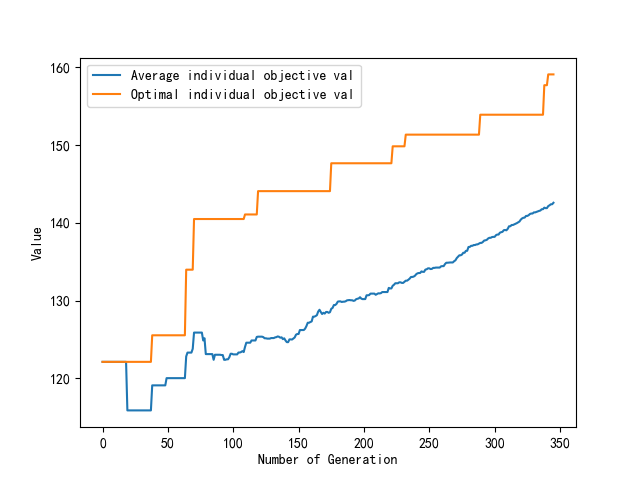
\includegraphics[width=0.46\columnwidth]{pic/convergence_4-16_n10_ep0.6_T500.png}
    }
    % \subfigure[$(\epsilon=0.6, T=750)$]{
    %     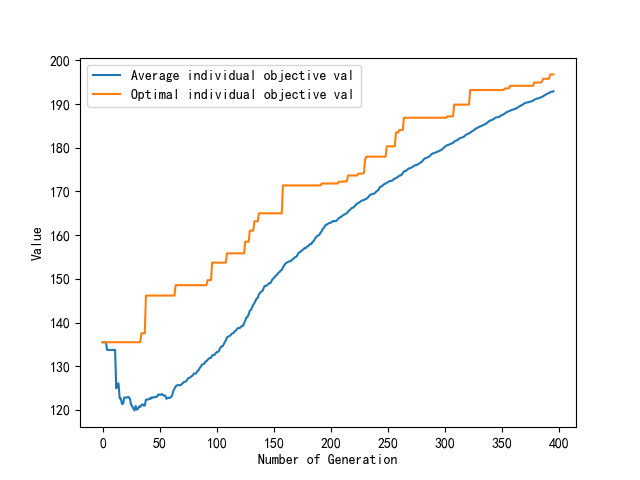
\includegraphics[width=0.46\columnwidth]{pic/convergence_4-16_n10_ep0.6_T750.png}
    % }
    \subfigure[$(\epsilon=0.6, T=1000)$]{
        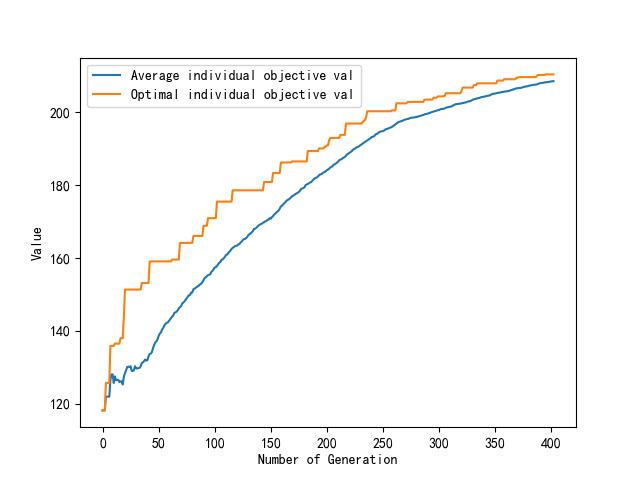
\includegraphics[width=0.46\columnwidth]{pic/convergence_4-16_n10_ep0.6_T1000.png}
    }
    \caption{Convergence Results of Differential Evolution Algorithm under Different $(\epsilon, T)$ on Apr. $16^{\rm th}$ with $n=10$}
    \label{fig:Convergence}
\end{figure}

As is shown in Figure 6, we can discover that for the larger $T$ with more relaxtion constraints, the optimal value could be obtained with less convergence steps.


% \subsubsection{Relationship between decision making $c_{ij}^* / c_{ij}^{max}$ and the airline capacity $c_{ij}^{max}$}
% In section 4.2.1 and 4.2.2, we have discussed thoroughly how the parameters affect our experimental results. But there still remains a question that $c_{ij}^{max}$ in some city pairs has small value, which can impose restrictions on our optimized value to zero. With this regard, we choose two different values of $c_{ij}^{max}$ among our constructed airline network. As presented in figure 5, more proportional number of flights will be cut with higher $c_{ij}^{max}$ under the same severity of pandemic. It may Probably due to the fact that more flights can't be satisfied under this level of severity and result in smaller $c_{ij}^* / c_{ij}^{max}$.



% \begin{figure}[H]
%     \centering
%     \subfigure[$c_{ij}^{max} = 20$]{
%         \includegraphics[width=0.46\columnwidth]{pic/decision_3-27_T_1000_ep_0dot75_max_20.eps}
%     }
%     \subfigure[$c_{ij}^{max} = 40$]{
%         \includegraphics[width=0.46\columnwidth]{pic/decision_3-27_T_1000_ep_0dot75_max_40.eps}
%     }
%     \caption{Decision making $c_{ij}^* / c_{ij}^{max}$ under different max capacity $c_{ij}^{max}$ on Mar. 27$^{\rm th}$ ($\epsilon=0.75,T=1000$)}
%     \label{fig:my_label}
% \end{figure}





% \subsection{Analysis}

% \begin{itemize}
%     \item Reasonable explanation for the “Five One” policy
%     \item The impact of the severity of the epidemic $S_i$ on decision making
%     \item The impact of airline capacity $c_{ij}^{max}$ on decision making
%     \item The impact of relaxation parameters $T$ and $\epsilon$ on decision making
% \end{itemize}




% =================================

